\documentclass[a4paper]{article}

\usepackage{inputenc}
\usepackage[british,UKenglish]{babel}
\usepackage{amsmath}
%\usepackage{titlesec}
\usepackage{color}
\usepackage{graphicx}
\usepackage{fancyref}
\usepackage{hyperref}
\usepackage{float}
\usepackage{scrextend}
\usepackage{setspace}
\usepackage{xargs}
\usepackage{multicol}
\usepackage{nameref}

\usepackage{sectsty}
\usepackage{multicol}
\usepackage{multirow}
\usepackage[procnames]{listings}
\usepackage{appendix}

\newcommand\tab[1][1cm]{\hspace*{#1}}
\hypersetup{colorlinks=true, linkcolor=black}
\interfootnotelinepenalty=10000

\newcommand{\cleancode}[1]{\begin{addmargin}[3em]{3em}\texttt{\textcolor{cleanOrange}{#1}}\end{addmargin}}
\newcommand{\cleanstyle}[1]{\text{\textcolor{cleanOrange}{\texttt{#1}}}}


\usepackage[colorinlistoftodos,prependcaption,textsize=footnotesize]{todonotes}
\newcommandx{\commred}[2][1=]{\textcolor{Red}
{\todo[linecolor=red,backgroundcolor=red!25,bordercolor=red,#1]{#2}}}
\newcommandx{\commblue}[2][1=]{\textcolor{Blue}
{\todo[linecolor=blue,backgroundcolor=blue!25,bordercolor=blue,#1]{#2}}}
\newcommandx{\commgreen}[2][1=]{\textcolor{OliveGreen}{\todo[linecolor=OliveGreen,backgroundcolor=OliveGreen!25,bordercolor=OliveGreen,#1]{#2}}}
\newcommandx{\commpurp}[2][1=]{\textcolor{Plum}{\todo[linecolor=Plum,backgroundcolor=Plum!25,bordercolor=Plum,#1]{#2}}}

\def\code#1{{\tt #1}}

\def\note#1{\noindent{\bf [Note: #1]}}

\makeatletter
%% The "\@seccntformat" command is an auxiliary command
%% (see pp. 26f. of 'The LaTeX Companion,' 2nd. ed.)
\def\@seccntformat#1{\@ifundefined{#1@cntformat}%
   {\csname the#1\endcsname\quad}  % default
   {\csname #1@cntformat\endcsname}% enable individual control
}
\let\oldappendix\appendix %% save current definition of \appendix
\renewcommand\appendix{%
    \oldappendix
    \newcommand{\section@cntformat}{\appendixname~\thesection\quad}
}
\makeatother


% "define" Scala
\usepackage[T1]{fontenc}
\usepackage{beramono}
\usepackage{microtype}

\sbox0{\small\ttfamily A}
\edef\mybasewidth{\the\wd0 }

\lstdefinelanguage{scala}{
  morekeywords={abstract,case,catch,class,def,%
    do,else,extends,false,final,finally,%
    for,if,implicit,import,match,mixin,%
    new,null,object,override,package,%
    private,protected,requires,return,sealed,%
    super,this,throw,trait,true,try,%
    type,val,var,while,with,yield},
  sensitive=true,
  morecomment=[l]{//},
  morecomment=[n]{/*}{*/},
  morestring=[b]",
  morestring=[b]',
  morestring=[b]"""
}

\usepackage{color}
\definecolor{dkgreen}{rgb}{0,0.6,0}
\definecolor{gray}{rgb}{0.5,0.5,0.5}
\definecolor{mauve}{rgb}{0.58,0,0.82}

% Default settings for code listings
\lstset{frame=tb,
  language=scala,
  aboveskip=3mm,
  belowskip=3mm,
  showstringspaces=false,
  columns=fixed, % basewidth=\mybasewidth,
  basicstyle={\small\ttfamily},
  numbers=none,
  numberstyle=\footnotesize\color{gray},
  % identifierstyle=\color{red},
  keywordstyle=\color{blue},
  commentstyle=\color{dkgreen},
  stringstyle=\color{mauve},
  frame=single,
  breaklines=true,
  breakatwhitespace=true,
  procnamekeys={def, val, var, class, trait, object, extends},
  procnamestyle=\ttfamily\color{red},
  tabsize=2
}

\lstnewenvironment{scala}[1][]
{\lstset{language=scala,#1}}
{}
\lstnewenvironment{cpp}[1][]
{\lstset{language=C++,#1}}
{}
\lstnewenvironment{bash}[1][]
{\lstset{language=bash,#1}}
{}
\lstnewenvironment{verilog}[1][]
{\lstset{language=verilog,#1}}
{}


\usepackage{style/pythonhighlight}
\lstset{frame=, basicstyle={\footnotesize\ttfamily}}


\usepackage{draftwatermark}
\SetWatermarkText{贪心科技版权所有}
\SetWatermarkScale{0.15}
\includegraphics{main}

\graphicspath{ {images/} }
\usepackage{ctex}
%-----------------------------------------BEGIN DOC----------------------------------------
\renewcommand{\baselinestretch}{1.5}

\begin{document}

\renewcommand{\contentsname}{目\ 录}
\renewcommand{\appendixname}{附录}
\renewcommand{\appendixpagename}{附录}
\renewcommand{\refname}{参考文献}
\renewcommand{\figurename}{图}
\renewcommand{\tablename}{表}
\renewcommand{\today}{\number\year 年 \number\month 月 \number\day 日}

\title{{\Huge 京东-贪心NLP项目实验手册{\large\linebreak\\}}{\Large 项目1:基于京东图书的文本分类\linebreak\linebreak}}
%please write your name, Student #, and Class # in Authors, student ID, and class # respectively
\author{\\项目设计和编写 : 修晔良\ 姜冰钰 \\
后期编辑: 李文哲\\
单\ 位: 贪心科技}
\date{\today}
\maketitle
\newpage


%-----------------------------------------ABSTRACT-------------------------------------

%-----------------------------------------CONTENT-------------------------------------
\begin{center}
\tableofcontents\label{c}
\end{center}
\newpage

\section{项目描述与目标}

\noindent 文本分类作为自然语言处理领域最经典的技术之一,有着非常广泛的应用,如情感分析、情绪识别、主题分类等等。文本分类任务通常分为两大类,\textbf{单标签分类}任务和\textbf{多标签分类}任务。\texttt{单标签分类任务}指的是对于一个输入文本,我们需要输出其中的一个类别。举个例子,我们把每一篇新闻分类成一个主题(如体育或者娱乐)。相反,\texttt{多标签分类任务}指的是对于一个输入文本,输出的类别有多个,如对应一篇新闻可以同时输出多个类别:体育、娱乐和音乐。其中,单标签任务又可以分为\textbf{二元(binary)分类}和\textbf{多类别分类} ,\texttt{二元分类}指的是只有两种不同的类别。 \\

\noindent 在本项目中,我们主要来解决文本单标签的任务。数据源来自于京东电商,任务是\textit{基于图书的相关描述和图书的封面图片,自动给一个图书做类目的分类}。这种任务也叫作\texttt{多模态分类} 。在现实应用中,为了解决一个问题,我们通常会面对多种类型的数据。比如在自动驾驶,为了有效操控车辆的方向,我们可以借助于传感器数据的同时也可以借助于摄像头的数据。\\

\noindent 通过本项目的练习,你能通晓机器学习建模的各个流程:
\begin{itemize}
    \item \textbf{文本的清洗和预处理} :这是所有 NLP 项目的前提,或多或少都会用到相关的技术。
    \item \textbf{文本特征提取}:任何建模环节都需要特征提取的过程,你将会学到如何使用\texttt{tfidf}、\textt{常用的词向量}~\cite{bojanowski2017enriching}、\texttt{FastText}~\cite{mikolov2013efficient}等技术来设计文本特征。
    \item \textbf{图片特征提取}:由于项目是多模态分类,图片数据也是输入信号的一部分。你可以掌握如何通过预训练好的\texttt{CNN}~\cite{DBLP:journals/corr/Kim14f}来提取图片的特征,并且结合文本向量一起使用。
    \item \textbf{模型搭建}:在这里你将会学到如何使用各类经典的机器学习分类模型来搭建算法,其中也会涉及到各种调参等技术。除此之外,处理样本不均衡也是一个非常现实且具有挑战的问题。
    \item \textbf{结果的可视化}:很多模型目前都是黑盒子,很难去理解背后的原因。通过本项目的练习,你将有机会掌握如何对一个复杂模型的结果做一些可视化分析,试图理解背后分类正确或者分类错误的原因。 
    \item \textbf{模型的部署}:工作的最后一般都会涉及到模型的部署,在这里你将会学到如何使用 Flask 等工具来部署模型。
\end{itemize}

\noindent 同时, 通过本项目
\begin{itemize}
    \item 1.  熟练掌握分词, 过滤停止词等技术
    \item 2.  熟练掌握训练、使用\texttt{tfidf}、\textt{word2vec}、\textt{fasttext}模型
    \item 3.  熟练掌握训练\texttt{Xgboost}模型, 以及常用评价指标, 并熟练掌握\texttt{Grid Search}调参方法
    \item 4.  熟练掌握使用\texttt{Flask}部署模型
    \item 5.  了解如何处理不均衡分类问题
    \item 6.  了解如何获取词性、命名实体识别结果
    \item 7.  了解如何使用\texttt{Resnet}、\texttt{Bert}、\texttt{Xlnet}等预训练模型获取embedding
    \item 8.  了解完整的深度学习模型代码架构
    \item 9.  了解如何使用\texttt{AE}获取词嵌入表示
    \item 10. 了解什么是可解释性模型
\end{itemize}

\noindent 作为第一个项目,我们的目标是希望帮助大家能够搭建起一个比较完善的文本分类系统,之后遇到类似的任何问题,都可以有能力去攻克。
\section{项目数据描述}

\begin{figure}[ht]
 \centering
 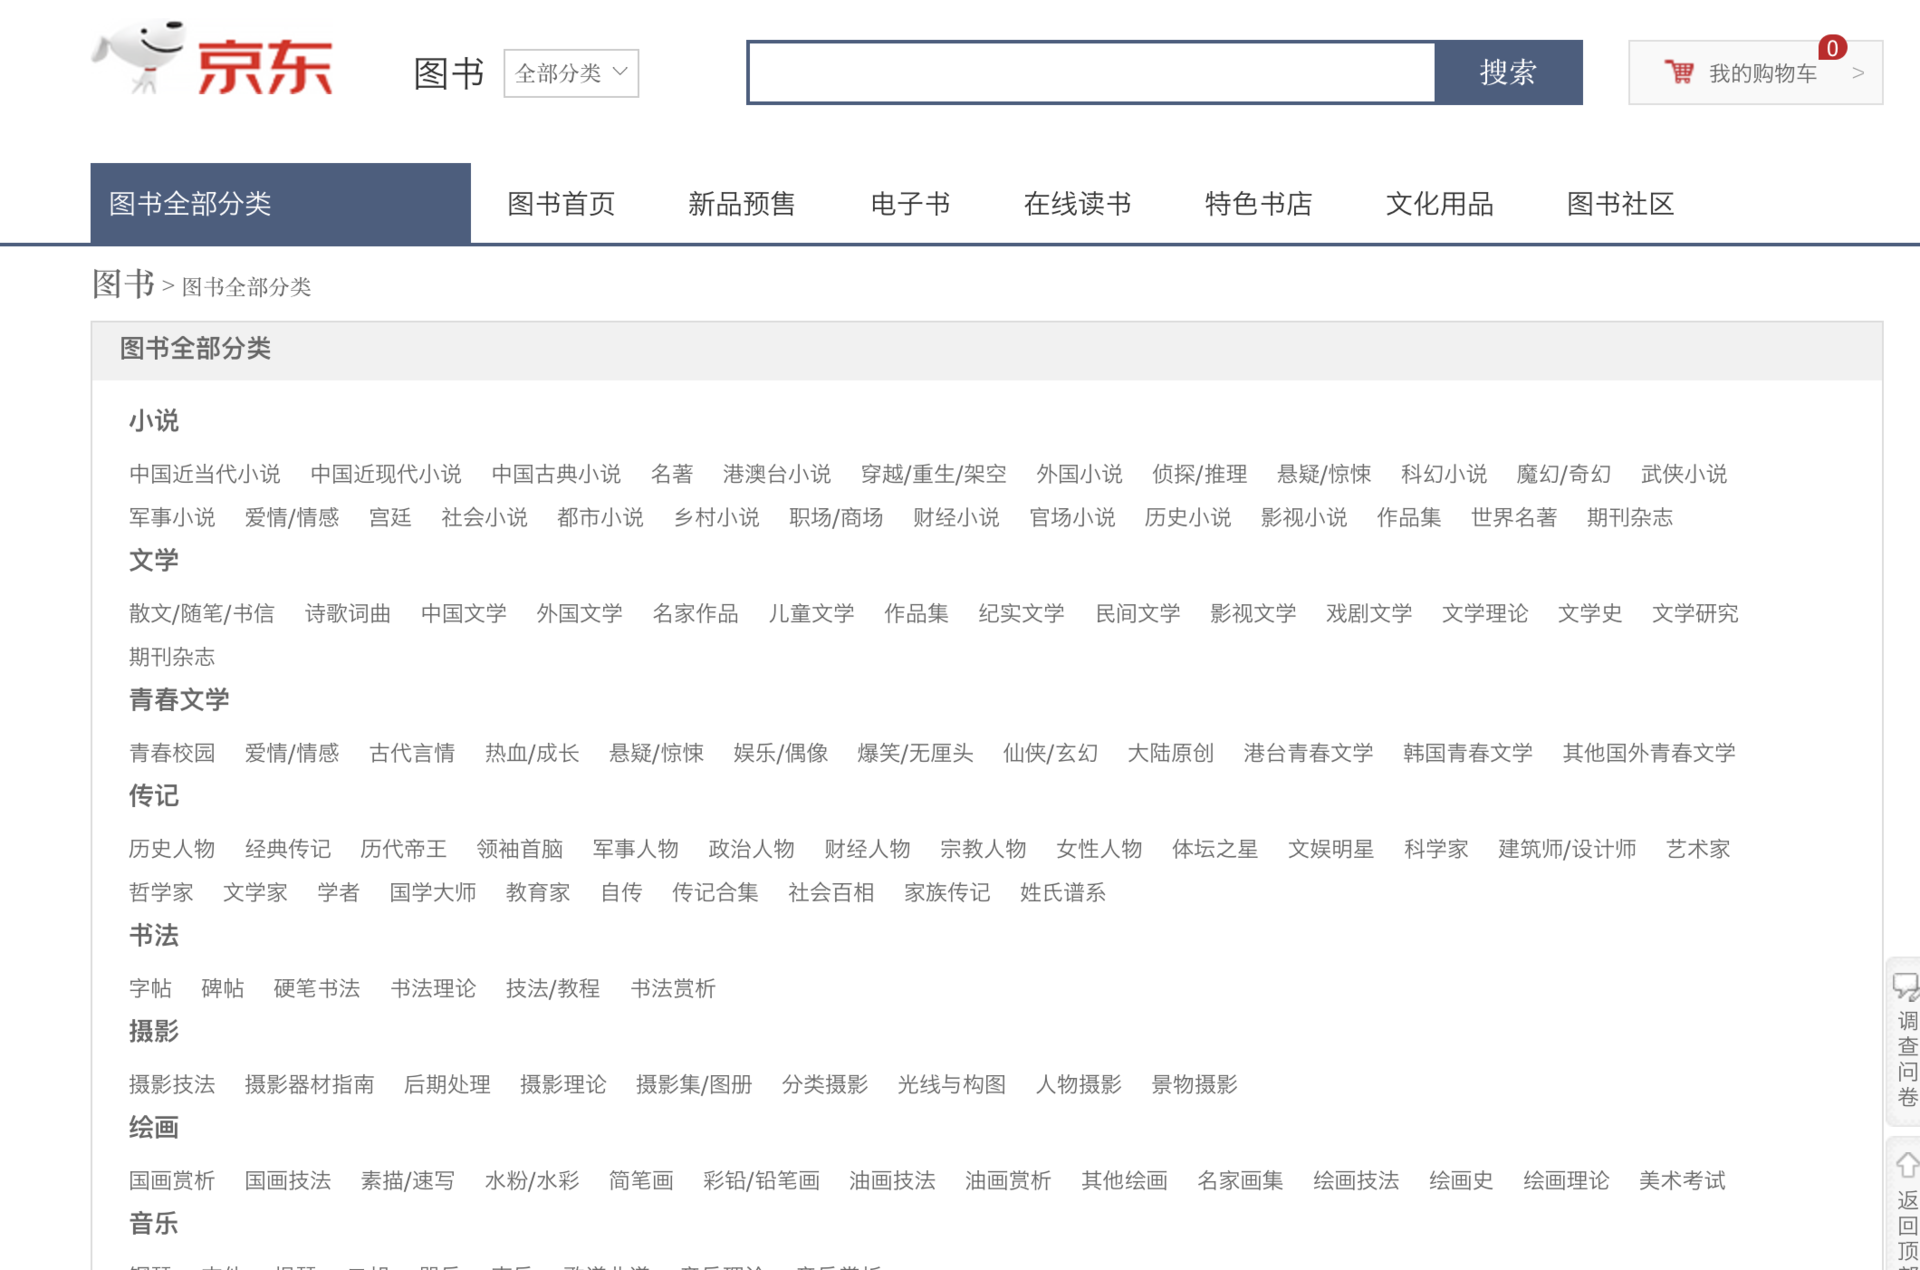
\includegraphics[height=8cm]{images/jd_book.jpg}
 \caption{京东图书类别\footnote{https://book.jd.com/booksort.html}}
 \label{fig:jd_book}
\end{figure}

\begin{figure}[ht]
 \centering
 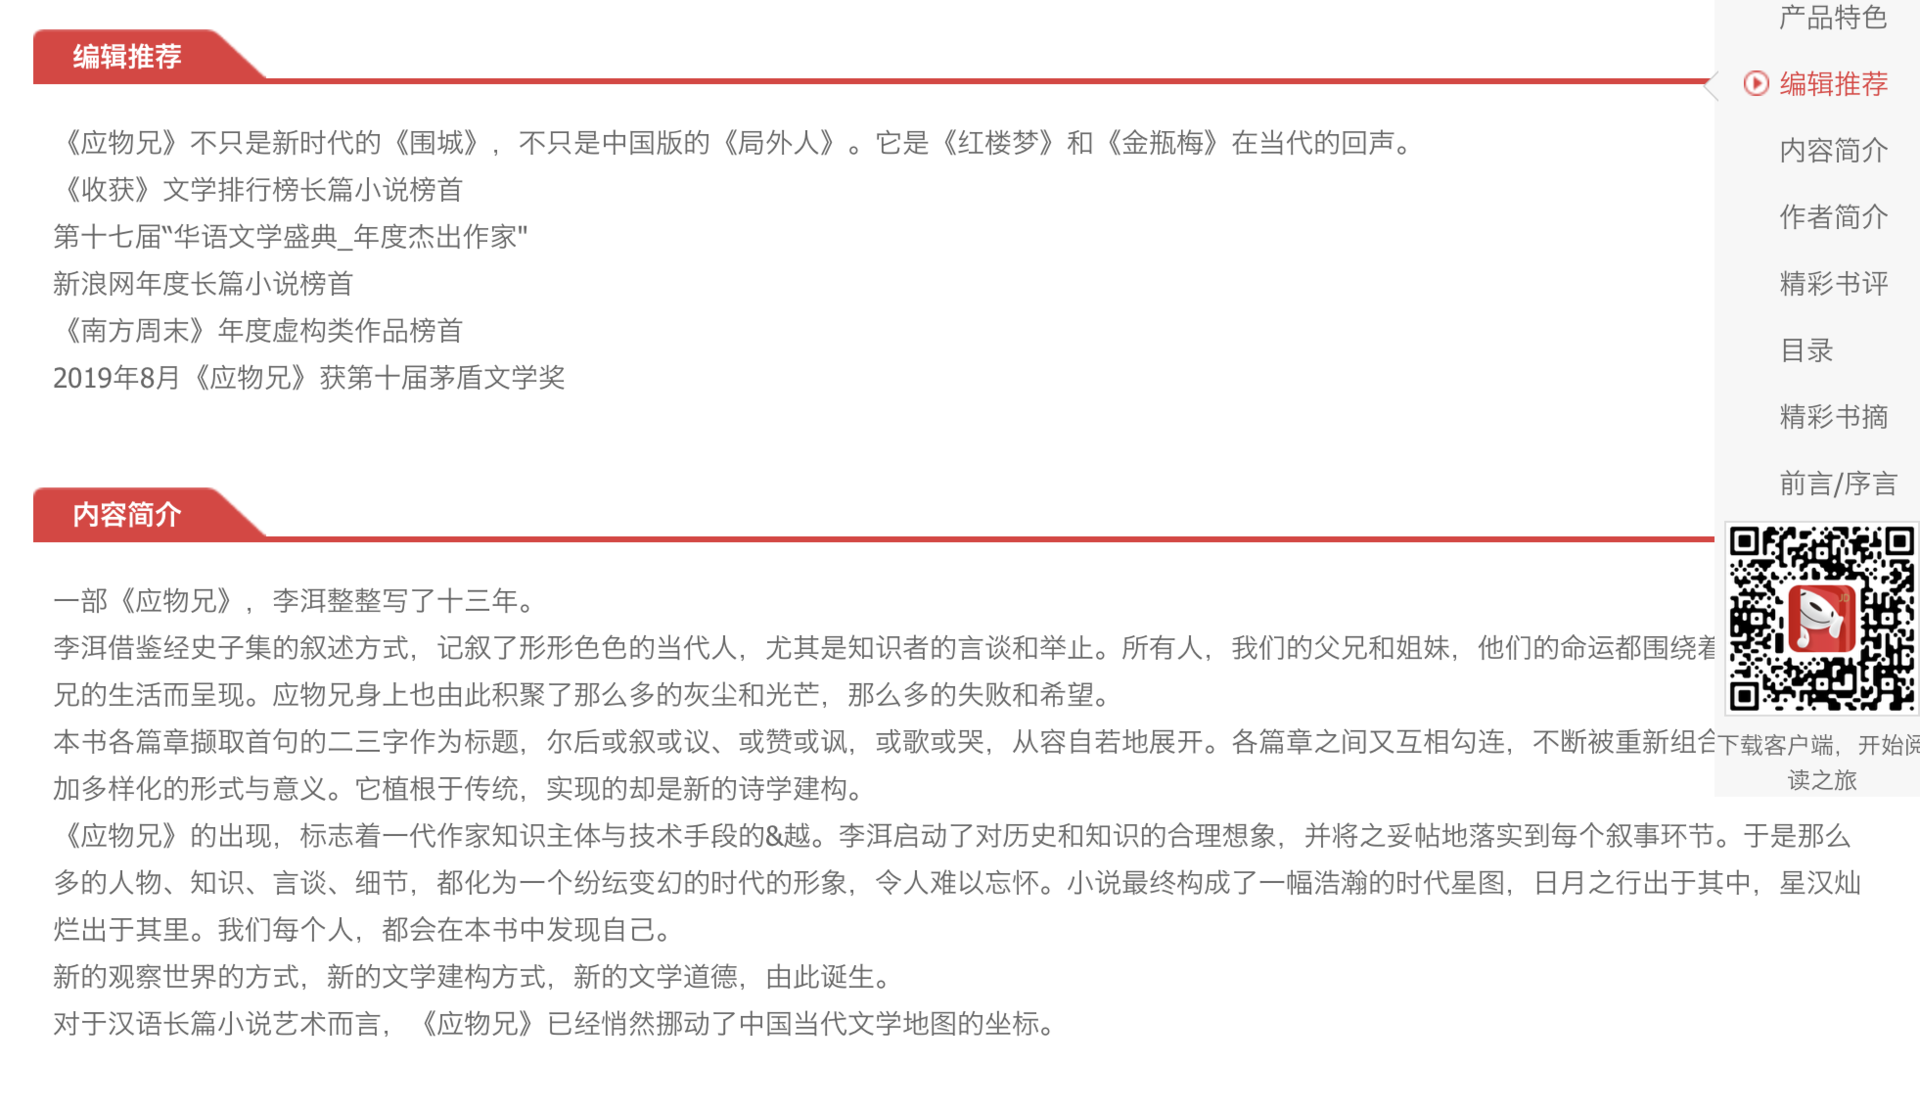
\includegraphics[height=7cm]{images/jd_book_text.jpg}
 \caption{京东图书内容简介}
 \label{fig:jd_book_text}
\end{figure}

\begin{figure}[ht]
 \centering
 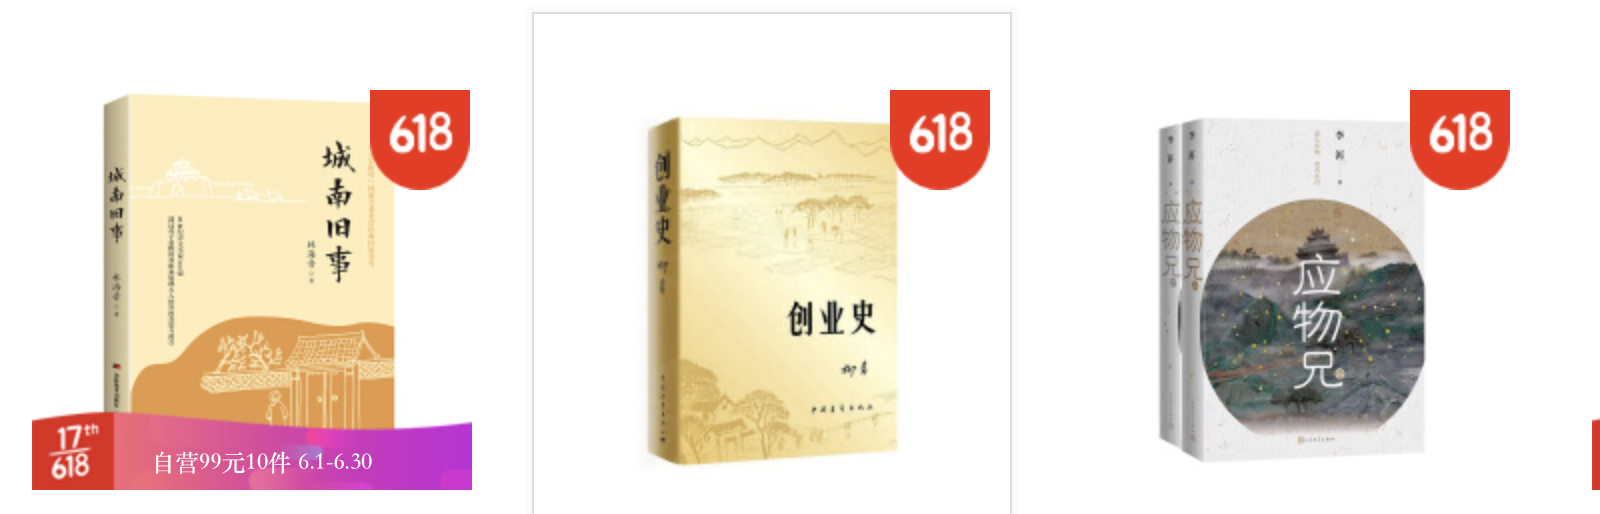
\includegraphics[height=4cm]{images/jd_book_cover.jpg}
 \caption{京东图书封面实例}
 \label{fig:jd_book_cover}
\end{figure}

\noindent 在本项目中,我们使用的是京东图书数据。在京东网站上,每一本图书都录属于列表中的一个类目,如图~\ref{fig:jd_book}所示。由于本项目中需要实现的是单标签多类别的分类模型,我们决定使用\textbf{图书的二级类目}作为样本的真实标签,比如“中国文学”,“纪实文学”,“青春校园”等。在给定的数据集中,一共包含$33$个不同类别的标签。\\

\noindent 对于标签的识别,我们使用两种类型的数据,分别为图书的文本内容简介(如图~\ref{fig:jd_book_text}所示)以及图书的封面图(如图~\ref{fig:jd_book_cover}所示)。\\

\nooindent 本项目使用的数据集中,一共包括206316个训练样本,58948个验证样本,29474个测试样本。
\section{项目事宜}

\noindent 本项目是基于图书的文本信息和图片信息来解决文本多分类任务。一般的AI项目流程可分为\textit{数据预处理、文本特征工程、建模和调参、评估以及部署构成}。通过本项目的实操,你将会体会到每个环节的细节如何去落地。



\subsection{项目的整个框架}

\noindent 整个项目框架如图~\ref{fig:project_mindmap}所示。下面对于图中每个模块做简要的描述,具体的细节请参考本文章后续的内容。

\begin{figure}[ht]
 \centering
 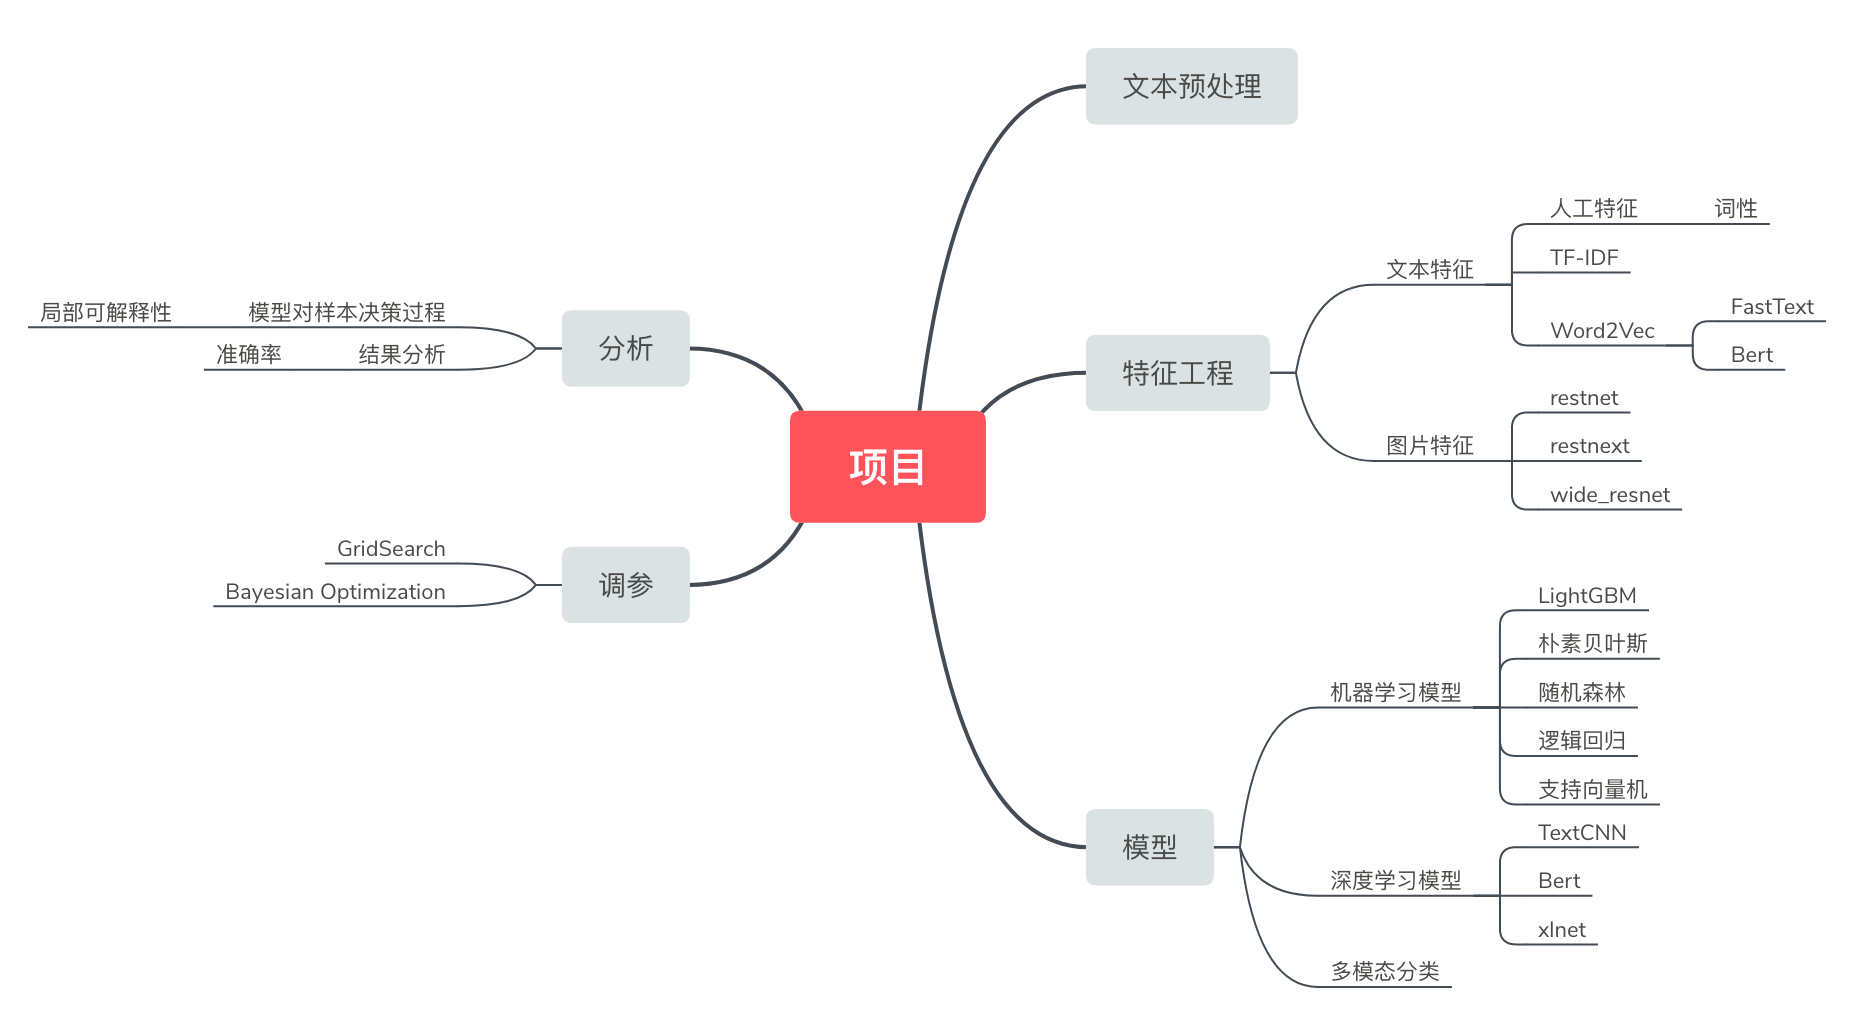
\includegraphics[height=7cm]{images/project_mindmap.jpg}
 \caption{京东图书分类项目模块架构图}
 \label{fig:project_mindmap}
\end{figure}

\begin{itemize}
    \item \textbf{特征工程}:这块涉及到文本和图片的特征。对于文本的特征,在本项目中需要使用\texttt{tf-idf~\cite{paik2013novel}}, 经典的预训练词向量(\texttt{FastText}, \texttt{BERT~\cite{DBLP:journals/corr/abs-1810-04805}})、以及人工抽取的一些特征如单词的词性、实体类别等。对于图片,我们将使用\texttt{ResNet~\cite{DBLP:journals/corr/HeZRS15}}等预训练模型来获得图片向量。等获取完文本和图片向量之后,我们会做特征的拼接来做多模态的训练。 
    \item \textbf{模型}:在训练过程中,你将有机会尝试使用各类经典的机器学习模型以及深度学习模型。很多模型已经提供给了大家,大部分模型不需要自己编写。  
    \item \textbf{调参}:对于模型的调参环节,我们选择使用\texttt{网格搜索}和\texttt{贝叶斯优化}搜索算法。后者相比前者可以缩小搜索空间,但同时也会增加每次的搜索代价,具体效率可以通过实验来体会。
    \item \textbf{分析}:评估模型的好坏通常都需要一个标准如准确率或者\texttt{F1-Score}。除此之外,目前对于深度学习模型来讲,很多时候都以黑盒子的形态来存在,我们很难判断为什么这个模型对于某些样本分类的很准确,对于某些样本分类错误。为了了解更多内部的机理,我们\textit{实现了基于词、短语以及词与词、短语与短语之间交互的可解释性模型},即针对一个样本,找出该样本中哪些词或者词组对模型分类的贡献度较大。
    \item \textbf{数据的不平衡处理}:另外,项目数据本身的类别不平衡:有些类别很多,有些类别则比较少,这对于训练模型来讲会有一定的挑战。项目中将使用\texttt{BalancedBaggingClassifier}、\texttt{SMOTE~\cite{DBLP:journals/corr/abs-1106-1813}} 和\texttt{ClusterCentroids}[3]等模型来解决上述问题。
\end{itemize}









\section{项目作业描述}

\noindent 任何 AI 项目通常包含\texttt{数据清洗、特征提取、建模、评估}以及\texttt{部署}的环节。所以本项目的安排也遵循此框架。由于具体涉及到的内容偏多,我们将会把上述项目\textbf{分成3个任务}来给到大家,由浅入深。在第一个任务中,大家需要用到经典的方法先搭建完整的流程,而且能够看到效果,类似于精益创业中的MVP(minimum value product)版本。在之后的第二个、第三个任务中,我们会逐步完善项目,最后并部署到线上。 

\subsection{第一次作业}
\noindent 作为第一个任务,我们希望帮助大家尽快搭建一个完整的流程,能在最短时间内看到效果。所以在第一个任务中,我们所采用的都是经典的方法论。第一次作业的框架图如图\ref{fig:book_task1_mindmap}所示。

\begin{figure}[ht]
 \centering
 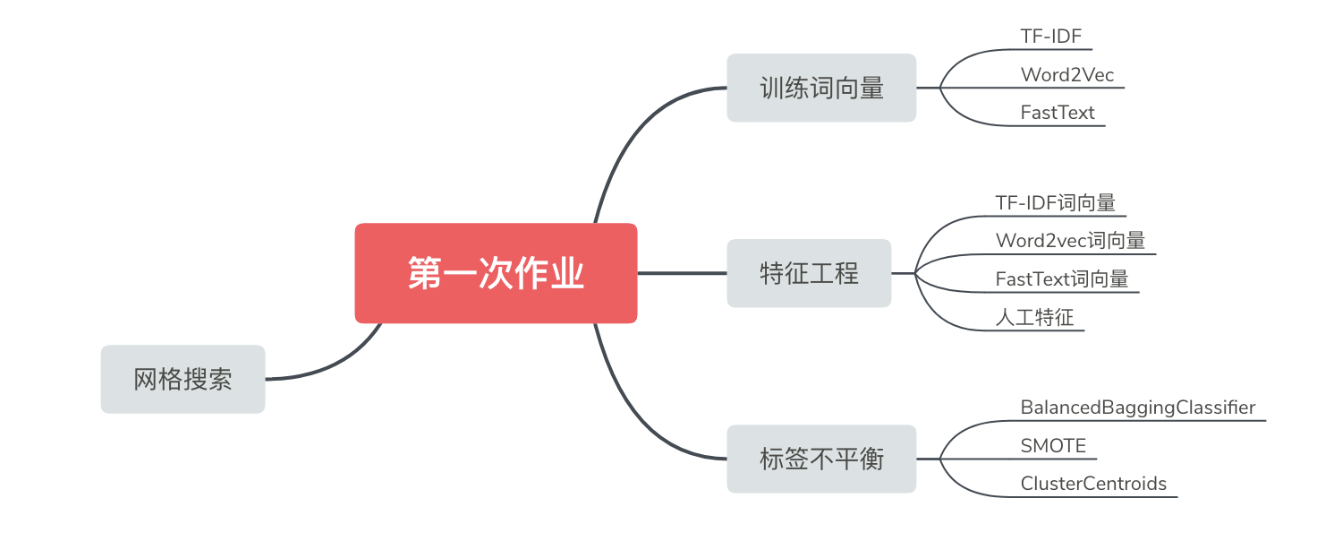
\includegraphics[height=5cm]{images/book_task1_mindmap}
 \caption{第一次作业架构图}
 \label{fig:book_task1_mindmap}
\end{figure}

\subsection{第一次作业描述}
\noindent 对于本次任务,需要完成如下的部分:
\begin{itemize}
    \item 第一:利用 TF-IDF、Word2Vec~\cite{DBLP:journals/corr/MikolovSCCD13}、FastText 等模型训练出词向量并训练传统机器学习模型
    \item 第二:灵活使用文本领域的特征工程方法,为样本提炼出更精确的表示,并分析出这些额外的特征是否让机器学习模型(比如 GDBT~\cite{friedman2001greedy})的效果有所提升。
    \item 第三:处理数据中标签不平衡的问题
    \item 第四:使用 Grid Search 进行参数搜索优化
\end{itemize}


\subsubsection{第一次作业涉及到的相关技术}

\noindent \textbf{训练词向量}

\noindent 需要通过\texttt{TF-IDF}、\texttt{Word2vec}和 \texttt{FastText}方法来获取样本的词嵌入(\texttt{embedding})。实验中将所有的训练集,验证集和测试集拼接在一起训练,来获取词向量。
\begin{python}
self.data = pd.concat([
    pd.read_csv(root_path + '/data/train_clean.tsv', sep='\t'),
    pd.read_csv(root_path + '/data/dev_clean.tsv', sep='\t'),
    pd.read_csv(root_path + '/data/test_clean.tsv', sep='\t')
])
\end{python}

\noindent \texttt{TF-IDF}的特征可以通过\texttt{TfidfVectorizer}对象来训练。

\begin{python}
count_vect = TfidfVectorizer(
            stop_words=self.stopWords, max_df=0.6, ngram_range=(1, 2))
\end{python}


\noindent 对于\texttt{Word2Vec}和\texttt{FastText},我们可以通过调用 \texttt{gensim.models.Word2Vec()}和 \texttt{gensim.models.FastText()}来训练并获取对应的词向量。

\begin{python}
self.w2v = models.Word2Vec(min_count=2,
                            window=3,
                            size=300,
                            sample=6e-5,
                            alpha=0.03,
                            min_alpha=0.0007,
                            negative=15,
                            workers=4,
                            iter=10,
                            max_vocab_size=50000)
\end{python}

\noindent 训练完成后,将训练好的词向量进行存储,以待后续使用。

\begin{python}
logger.info('save tfidf model')
joblib.dump(self.tfidf, root_path +'/src/Embedding/models/tfidf_model')
logger.info('save word2vec model')
self.w2v.save(root_path + '/src/Embedding/models/w2v_model_50000')
\end{python}


\noindent\textbf{训练传统机器学习模型}

\noindent 在任务1中,我们使用了\texttt{随机森林模型、支持向量机、朴素贝叶斯、线性回归}和\texttt{GBDT}模型。这里以\texttt{GBDT} 模型为例进行一些说明:下面的表格~\ref{fig:book_task1_table1}\ref{fig:book_task1_table2}分别给出了传统机器学习模型分别在\texttt{word2vec}的原始词向量和\texttt{FastText} 的原始词向量上的准确率。根据实验结果分析发现,支持向量机模型的准确率最高,随机森林的准确率较低,随机森林模型可以通过调节超参数获得更高的准确率。另外,基于FastText的词向量表示的分类模型结果稍低于基于Word2vec的试验结果。这是由于Word2vec模型训练字典中有26119个词,而FastText模型中仅有19592个词。因此FastText构造的样本表示质量要稍低于Word2vec,从而导致基于FastText的分类结果略低于基于Word2vec的分类模型。

\begin{figure}[ht]
 \centering
 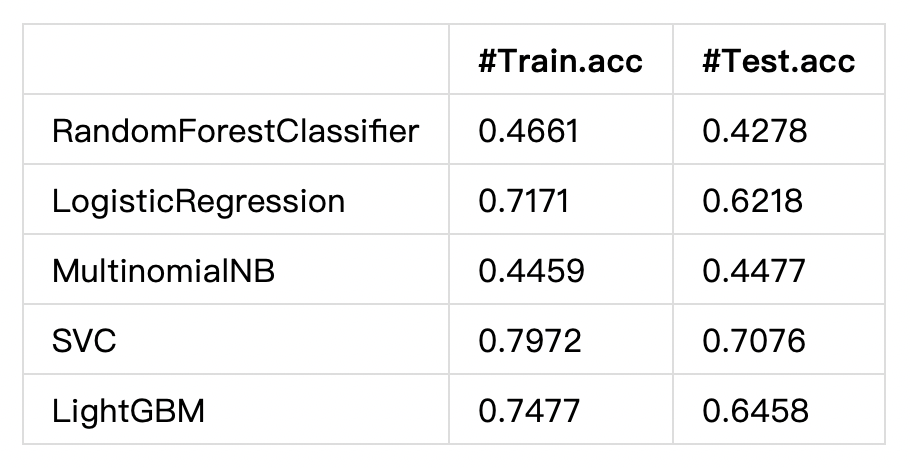
\includegraphics[height=4cm]{images/book_task1_table1.jpg}
 \caption{机器学习模型在word2vec向量中的\\}
 \label{fig:book_task1_table1}
\end{figure}

\begin{figure}[ht]
 \centering
 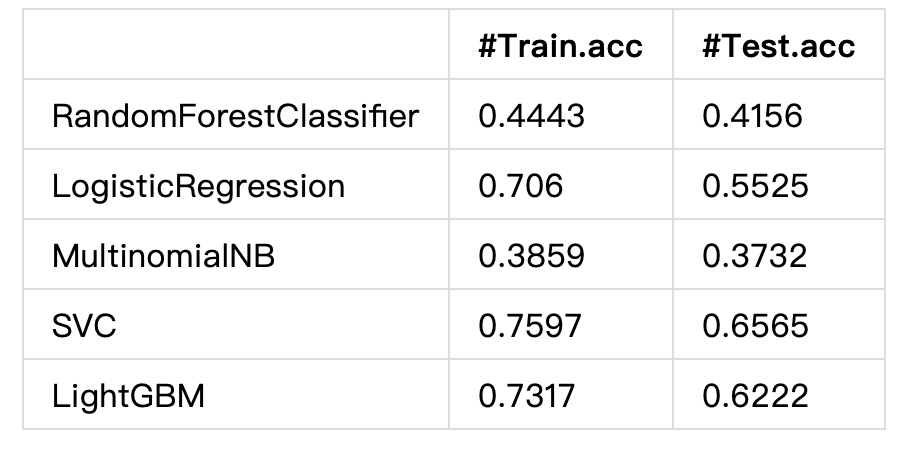
\includegraphics[height=4cm]{images/book_task1_table2.jpg}
 \caption{机器学习模型基于\texttt{Fast}的词向量分类精度\\}
 \label{fig:book_task1_table2}
\end{figure}


\noindent \textbf{特征工程}

\noindent 对于特征工程,我们做了如下两方面提取的操作:1.\textbf{基于词向量的特征工程} 2. \textbf{基于人工定义的特征}。\\

\noindent \textit{基于词向量的特征工程}主要包括以下几个方面:

\begin{itemize}
    \item 基于 \texttt{Word2vec}或者\texttt{FastText} 的词嵌入求出某个词向量的最大值和平均值,并把它们作为样本新的特征。
    \item 在样本表示中融合\texttt{Bert,XLNet~\cite{yang2019xlnet}}等预训练模型的\texttt{embedding}。
    \item 由于之前抽取的特征并没有考虑词与词之间交互对模型的影响,对于分类模型来说,贡献最大的不一定是整个句子, 可能是句子中的一部分, 如短语、词组等等。 在此基础上我们使用大小不同的滑动窗口(k=[2, 3, 4]), 然后进行平均或取最大操作。
    \item 在样本表示融合样本在自动编码器(AutoEncoder~\cite{bourlard1988auto})模型产生的 Latent features。
    \item 在样本表示融合样本在LDA~\cite{blei2003latent}模型产生的 Topic features。
    \item 将\texttt{Word2Vec、Fasttext} 词向量求和或取最大值
    \item 由于没有考虑类别的信息, 因此我们从训练好的模型中获取到所有类别的embedding, 与输入的word embedding矩阵相乘,对其结果进行 \texttt{softmax}运算,对\texttt{attention score} 与输入的word embedding 相乘的结果求平均或者取最大。具体架构示意图如图~\ref{fig:book_task1_feature_word}所示。 
\end{itemize}


\begin{figure}[ht]
 \centering
 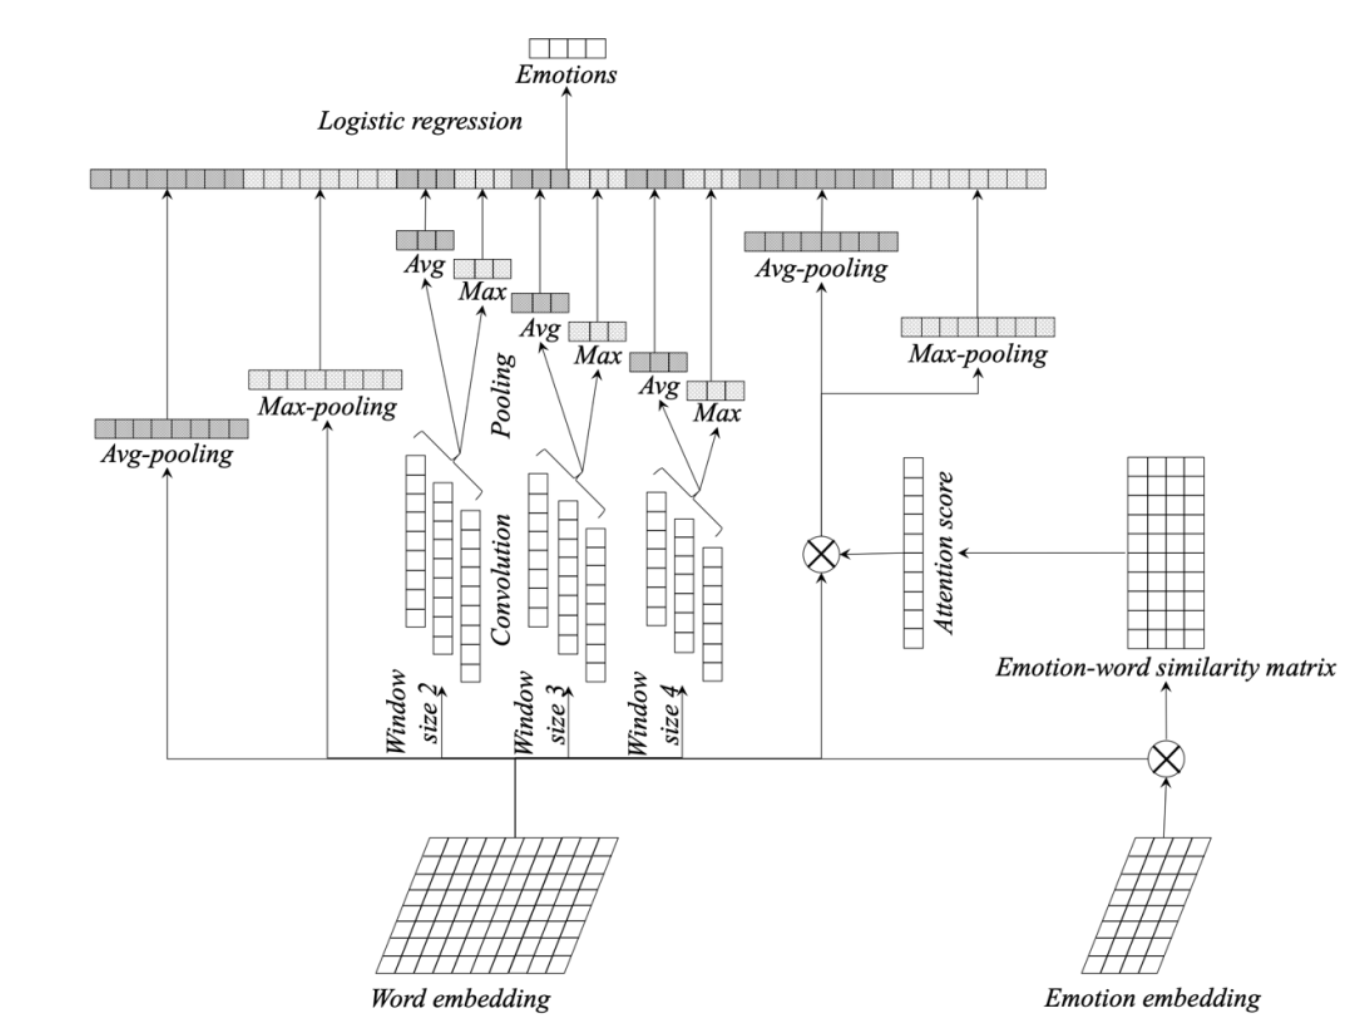
\includegraphics[height=10cm]{images/book_task1_feature_word.jpg}
 \caption{特征工程示意图\footnote{https://mp.weixin.qq.com/s/k-gS6k3-hy-ZI_r901IGvg}}
 \label{fig:book_task1_feature_word}
\end{figure}

\noindent 示例:

如input 为:\texttt{ "《应物兄》不只是新时代的《围城》,不只是中国版的《局外人》。"}, 分词后结果假设为:"《 应物兄 》 不 只是 新 时代 的 《 围城 》 , 不 只是 中国 版 的 《 局外人 》 。", 过滤掉停止词后结果假设为: \texttt{"应物兄 只是 新 时代 围城 只是 中国 版 局外人"},共计9个词。匹配我们已经训练好的\texttt{embedding}, 得到\texttt{9 * 300}维的向量。

因为input的句子长短是不一样的, 所以为了保证输入到模型的维度是相同的, 有两种方法: 1. 将长度的维度消去; 2. 将所以文本的的长度补至一样长。 第二种方法, 会增加不必要的计算量, 所以在此我们选择使用第一种方法。 使用\texttt{avg}, \texttt{max}的方法聚合, 得到300维的向量。

接下来我们使用类似\texttt{n-gram}的方法来获取词组, 短语级别的信息。如我们只考虑前面一个词, 得到结果为: "应物兄只是 只是新 新时代 时代围城 围城只是 只是中国 中国版 版局外人", \texttt{8 * 300} 或\texttt{8 * 2 * 300}维的向量。同样的方法我们将表示长度的维度消去(由于我们分别考虑前面2个词、3个词、4个词, 所以维度也是相同的, 可以不用消去,而是将2 * 300 转成1 * 600的向量,与其他特征拼接)。

由于我们的模型没有利用到label信息, label词大多出现在我们的数据集中, 我们考虑使用输入与label的相似程度来加权聚合我们的词向量。 首先,输入embedding(假设 9 * 300) 与 标签embedding (假设30 * 300)进行矩阵乘法, 得到(9 * 5)的矩阵。然后使用\texttt{avg、 max、 softmax等}聚合方法消去标签的维度, 其结果与输入embedding进行点乘, 并对得到加权后的结果聚合。 将所有特征拼接至一起,  输入至\texttt{Xgboost}模型训练。\\

\noindent \textit{基于人工定义的特征}包括以下几个方面:

\begin{itemize}
    \item 考虑样本中词的词性,比如句子中各种词性(名词,动词)的个数,从而使得构造的样本表示具有多样性,从而提高模型的分类精度。
    \item 通过命名实体识别的技术来识别样本中是否存在地名,是否包含人名等,可以将这些特征加入到样本特征中。
\end{itemize}


\noindent \textbf{标签不平衡处理}

\noindent 由于本项目数据集中的标签类别较多,但是不同类别样本的数量差异较大,即存在标签不平衡的情况。为了解决该问题,引入了 \texttt{BalancedBaggingClassifier}、\texttt{SMOTE}和 \texttt{ClusterCentroids}。

\noindent \textbf{方法一}:通过上采样的方法从原始数据集中抽样出平衡的数据集。

\begin{python}
from imblearn.over_sampling import SMOTE
X_resampled, y_resampled = SMOTE().fit_sample(Train_features, Train_label)
\end{python}

\noindent \textbf{方法二}:通过下采样的方法从原始数据集中抽样出平衡的数据集。

\begin{python}
from imblearn.under_sampling import ClusterCentroids
cc = ClusterCentroids(random_state=0)
X_resampled, y_resampled = cc.fit_sample(Train_features, Train_label)
\end{python}

\noindent \textbf{方法三}:通过集成的方法从原始数据集中抽样出样本标签平衡的数据集。


\begin{python}
from imblearn.ensemble import BalancedBaggingClassifier
print("通过 ensember 中集成的方法来处理不平衡的标签")
bbc = BalancedBaggingClassifier(base_estimator=RF_model,
                                sampling_strategy='auto',
                                replacement=False,
                                random_state=0)
\end{python}


\noindent \textbf{网格搜索超参数优化}\\

\noindent \texttt{GBDT}的实现有很多种,在此我们使用微软开发的\texttt{LightGBM~\cite{ke2017lightgbm}}。\texttt{GDBT} 的超参数较多,为了找到模型最优的超参数组合,我们在项目中使用基于网格搜索的超参数优化算法来实现交叉验证。\\

\noindent \textbf{1. 网格搜索}:网格搜索优化需要提前定义好各个超参数的范围,然后遍历所有超参数组成的笛卡尔积的参数集合。通常网格优化的时间复杂度较大,消耗时间较大。
\begin{python}
# 网格搜索
parameters = {
    'max_depth': [5, 10, 15, 20, 25],
    'learning_rate': [0.01, 0.02, 0.05, 0.1, 0.15],
    'n_estimators': [100, 500, 1000, 1500, 2000],
    'min_child_weight': [0, 2, 5, 10, 20],
    'max_delta_step': [0, 0.2, 0.6, 1, 2],
    'subsample': [0.6, 0.7, 0.8, 0.85, 0.95],
    'colsample_bytree': [0.5, 0.6, 0.7, 0.8, 0.9],
    'reg_alpha': [0, 0.25, 0.5, 0.75, 1],
    'reg_lambda': [0.2, 0.4, 0.6, 0.8, 1],
    'scale_pos_weight': [0.2, 0.4, 0.6, 0.8, 1]
}
gsearch = GridSearchCV(model, param_grid=parameters, scoring='accuracy', cv=3)
\end{python}

\subsection{第二次作业}

\noindent 第二个任务的主要工作是实现多模态模型,也就是加入图片信息的特征。另外,在第二个任务中,你需要使用贝叶斯超参数优化算法来解决优化问题,并且跟经典的网格搜索算法做比较。第二次作业的框架如图~\ref{fig:book_task2_mindmap}所示。 

\begin{figure}[ht]
 \centering
 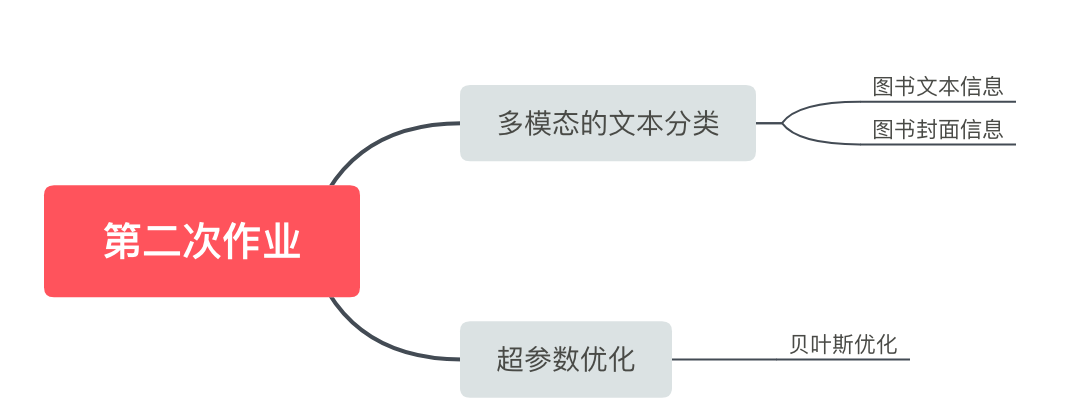
\includegraphics[height=4.5cm]{images/book_task2_mindmap.jpg}
 \caption{第二次作业思维导图}
 \label{fig:book_task2_mindmap}
\end{figure}


\subsubsection{第二次作业描述}

\noindent 对于本次任务,需要完成如下的思维导图部分。

\begin{itemize}
    \item \textbf{第一}:在第一个任务的基础上,融合图书样本的封面信息来实现多模态的文本多分类。
    \item \textbf{第二}:利用贝叶斯优化(\texttt{bayesian optimization~\cite{snoek2012practical}})来实现对模型超参数的优化。
\end{itemize}


\subsubsection{第二次作业涉及到的相关技术}


\noindent \textbf{实现多模态的文本多分类模型}

\noindent 对于图书,我们除了拥有文本信息~\ref{fig:book_task2_text}, 还拥有它的封面信息如图~\ref{fig:book_task2_cover}所示。我们希望把图书的特征信息也融合到模型当中,所以这里的核心问题是如何抽取图片的特征信息。 

\begin{figure}[ht]
 \centering
 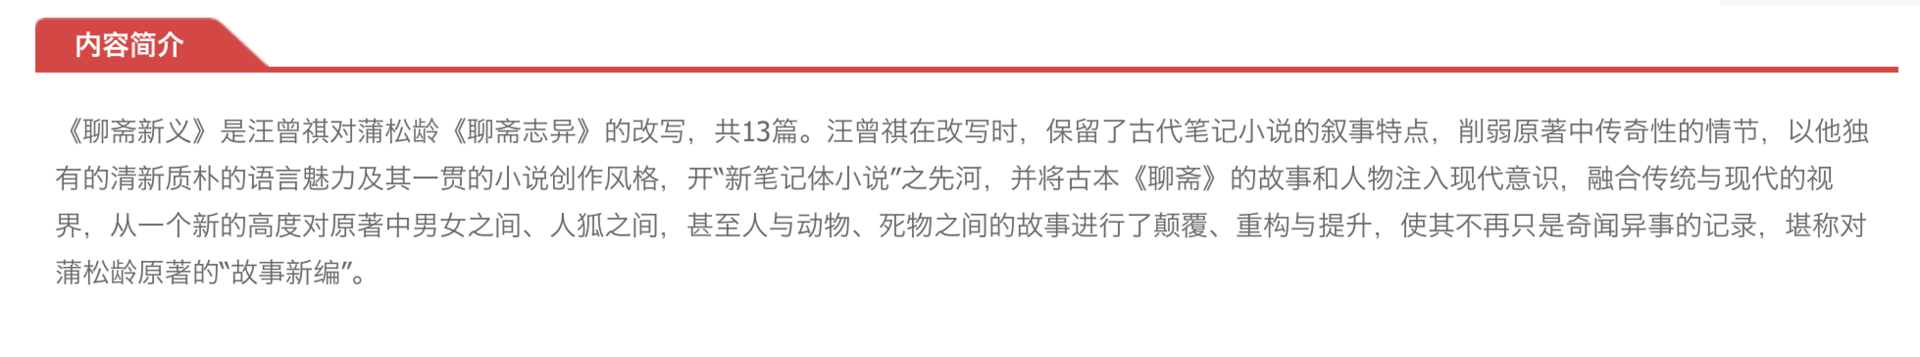
\includegraphics[height=2.6cm]{images/book_task2_text.jpg}
 \caption{图书的文本信息}
 \label{fig:book_task2_text}
\end{figure}

\begin{figure}[ht]
 \centering
 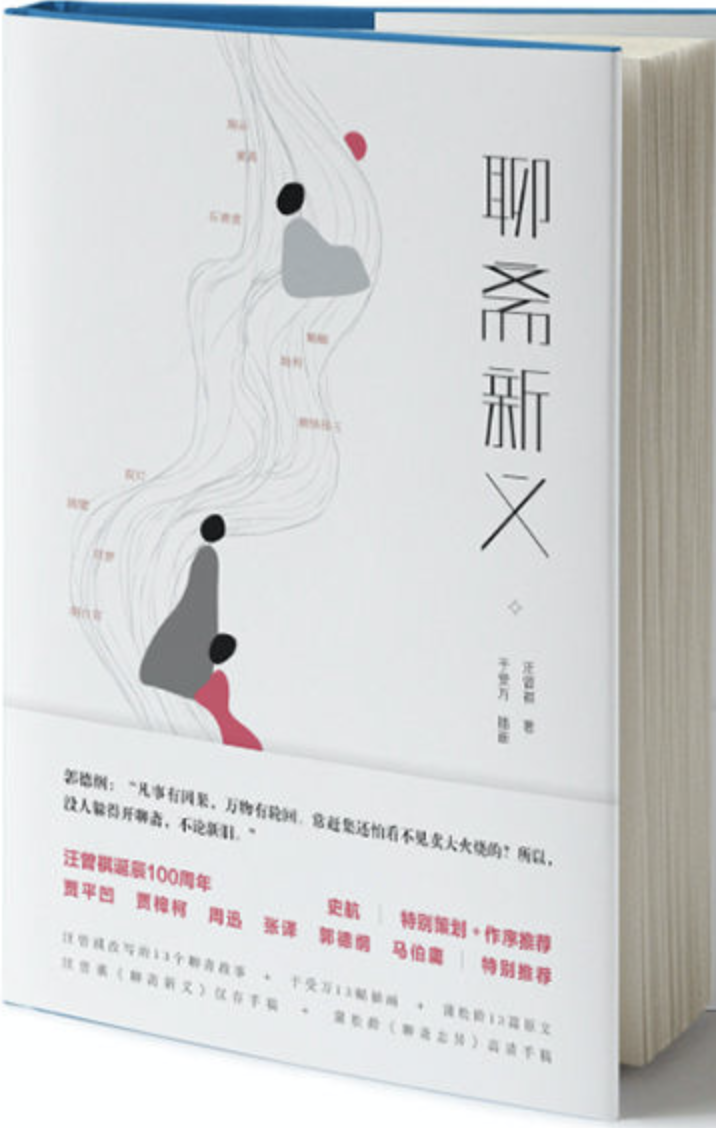
\includegraphics[height=4cm]{images/book_task2_cover.jpg}
 \caption{图书的封面信息}
 \label{fig:book_task2_cover}
\end{figure}
 
\noindent 对于图书的特征提取,我们考虑了各类\texttt{Pre-trained }模型,如\texttt{restnet、resnext~\cite{DBLP:journals/corr/XieGDTH16}、wide resnet~\cite{zagoruyko2016wide}}等\texttt{SOTA}模型。模型~\cite{kiela2019supervised}架构如图~\ref{fig:book_task2_transformer}所示。具体的实现细节,请参考实训平台的代码注解。\\

\begin{figure}[ht]
 \centering
 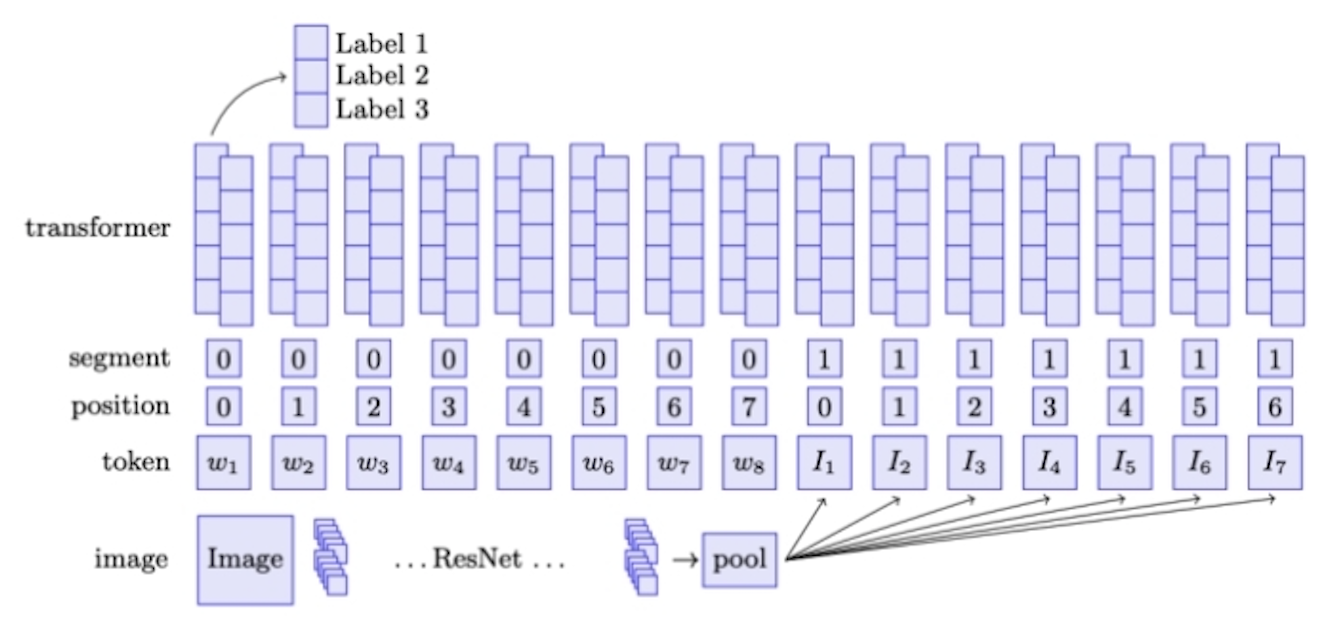
\includegraphics[height=6cm]{images/book_task2_transformer.jpg}
 \caption{图书封面特征信息的提取~\cite{tsai2019MULT}\\}
 \label{fig:book_task2_transformer}
\end{figure}\\

\begin{python} 
    class ImageEncoder(nn.Module):
    def __init__(self, args):
        super(ImageEncoder, self).__init__()
        self.args = args
        if self.args.pre-train == 'resnet':
            model = torchvision.models.resnet152(pretrained=True)
        elif self.args.pre-train == 'resnext101':
            model = torchvision.models.resnext101_32x8d(pretrained=True)
        elif self.args.pre-train == 'wide_resnet':
            model = torchvision.models.wide_resnet101_2(pretrained=True)
        modules = list(model.children())[:-2]
        self.model = nn.Sequential(*modules)

        pool_func = (
            nn.AdaptiveAvgPool2d
            if args.img_embed_pool_type == "avg"
            else nn.AdaptiveMaxPool2d
        )

        if args.num_image_embeds in [1, 2, 3, 5, 7]:
            self.pool = pool_func((args.num_image_embeds, 1))
        elif args.num_image_embeds == 4:
            self.pool = pool_func((2, 2))
        elif args.num_image_embeds == 6:
            self.pool = pool_func((3, 2))
        elif args.num_image_embeds == 8:
            self.pool = pool_func((4, 2))
        elif args.num_image_embeds == 9:
            self.pool = pool_func((3, 3))

    def forward(self, x):
        # Bx3x224x224 -> Bx2048x7x7 -> Bx2048xN -> BxNx2048
        out = self.pool(self.model(x))
        out = torch.flatten(out, start_dim=2)
        out = out.transpose(1, 2).contiguous()
        return out
\end{python}\\

\noindent \textbf{贝叶斯优化}
\noindent 基于贝叶斯优化的调参算法由J.Snoek(2012)提出。它的主要思想是,给定优化的目标函数(广义的函数,只需指定输入和输出即可,无需知道内部结构以及数学性质),通过不断地添加样本点来更新目标函数的后验分布(高斯过程,直到后验分布基本贴合于真实分布。简单的说,就是考虑了上一次参数信息,从而更好的调整当前的参数。\\
\begin{python} 
def Bayes_Optimization(Train_features4, Test_features4,                               Train_label4, Test_label4):
    rf_bo = BayesianOptimization(
        rf,
        {'n_estimators': (10, 2000),'max_depth': (4, 15),
         'reg_alpha': (0, 50),'reg_lambda': (0, 100),
         'learning_rate': (0.01, 0.1),
         'subsample': (0.1, 0.99)
         }
    )
    rf_bo.maximize()
\end{python}
\noindent 贝叶斯优化与常规的网格搜索或者随机搜索的区别是:贝叶斯调参采用高斯过程,考虑之前的参数信息,不断地更新先验;网格搜索未考虑之前的参数信息。贝叶斯调参迭代次数少,速度快;网格搜索速度慢,参数多时易导致维度爆炸;贝叶斯调参针对非凸问题依然稳健;\\

\subsection{第三次作业}

\noindent 第三次作业的核心目标是训练深度学习的分类模型,同时通过一种方式来解释深度学习模型。很多时候,我们把深度学习当作黑盒子来对待,其实不太清楚里面的运行机理。如一个样本被分类错误了,我们其实也不清楚为什么。为了解开模型内部的黑纱,需要一种方法来对内部做一些可解释性的操作。第三次作业框架如图~\ref{fig:book_task3_mindmap}所示。

\begin{figure}[ht]
 \centering
 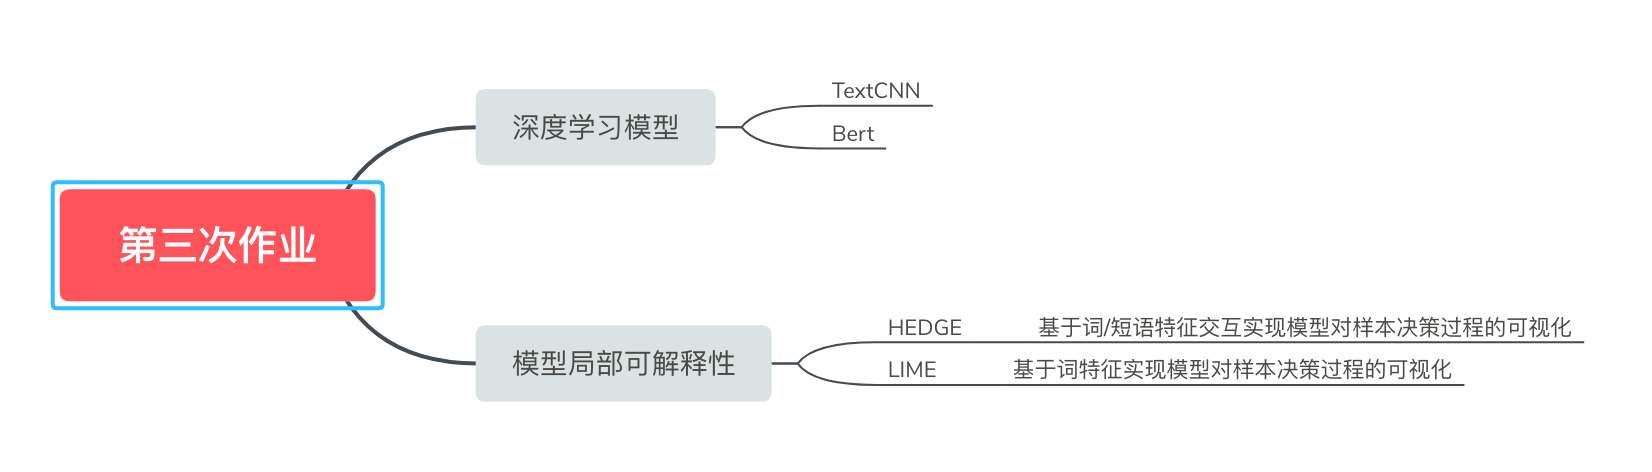
\includegraphics[height=4cm]{images/book_task3_mindmap}
 \caption{第三次作业架构图}
 \label{fig:book_task3_mindmap}
\end{figure}
\subsubsection{第三次作业描述}

\noindent 对于本次任务,需要完成如下的部分:
\begin{itemize}
\item \textbf{第一}:在第一次和第二次作业的基础上,实现文本分类的深度学习模型(比如 \texttt{TextCNN})。
\item \textbf{第二}:实现模型对样本的决策过程的可视化。
\end{itemize}

\subsubsection{第三次作业涉及到的相关技术}

\noindent \textbf{训练深度学习模型}\\

\noindent 在本项目中,我们实现了一些经典的深度学习方法,其中包括 \texttt{CNN}、\texttt{Bert} 等。利用\texttt{Pre-trained Bert}模型, 在图书案例上进行 \texttt{fine-tune}。对比实验结果可以发现,基于神经网络模型的分类效果一般要高于传统的机器学习模型的效果。\\

\begin{python}
class Model(nn.Module):
    def __init__(self, config):
        super(Model, self).__init__()
        model_config = BertConfig.from_pretrained(
            config.bert_path, num_labels=config.num_classes)
        self.bert = BertModel.from_pretrained(
            config.bert_path, config=model_config)
        for param in self.bert.parameters():
            param.requires_grad = True
        self.fc = nn.Linear(config.hidden_size, config.num_classes)


    def forward(self, x):
        context = x[0]  # 输入的句子
        # 对 padding 部分进行 mask,和句子一个 size,padding 部分用 0 表示,如:[1, 1, 1, 1, 0, 0]
        mask = x[1]
        token_type_ids = x[2]
        _, pooled = self.bert(context, attention_mask=mask,
                            token_type_ids=token_type_ids)
        out = self.fc(pooled)
        return o
\end{python}

\noindent \textbf{实现模型对样本决策的可解释性}

\noindent 神经网络模型通常被看成一个黑盒,比如在文本分类任务上,即很难直观上理解为什么样本会被模型预测为对应的类别。为了解决该问题,可以通过局部可解释性的方法来完成模型对样本预测结果的解释和可视化。局部可解释性主要是通过分析改变样本的特征从而导致样本预测结果变化的程度,如果该特征对样本决策影响较大的话,则说明该特征对样本分类起到关键作用,反之,如果该特征对样本预测结果的影响不大,则说明该特征对样本决策的贡献度较大。\\
\begin{figure}[ht]
 \centering
 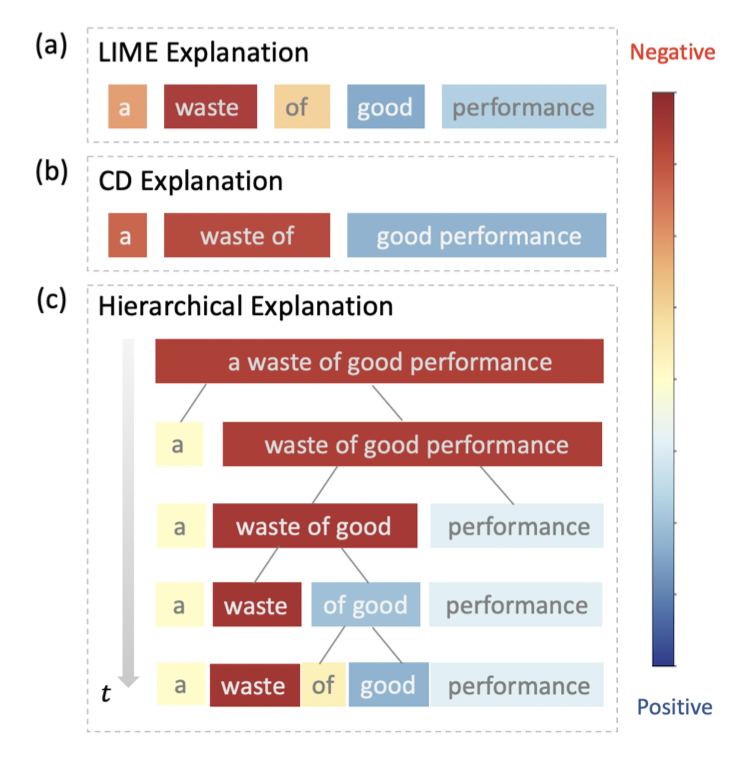
\includegraphics[height=9cm]{images/book_task3_interprete.jpg}
 \caption{文本分类中的局部可解释性~\cite{chen2020generating}}
 \label{fig:book_task3_interprete}
\end{figure}

\noindent 如图~\ref{fig:book_task3_interprete}所示,(a)显示的方法主要是分析在词级别上模型对样本决策的可解释性(LIME~\cite{DBLP:journals/corr/RibeiroSG16}),(b)给出了样本在分类模型下短语级别的可解释性,(c)给出了样本在分类模型下不同词或短语交互情况下的可解释性(HEDGE~\cite{chen2020generating})。以(a)为例进行说明,词的不同颜色体现了该词对样本在模型下分类预测成对应类的贡献度。

\bibliographystyle{acm}
\bibliography{reference}
\end{document}

